%=======================================================================
\chapter[Multi-paradigm programming in Prolog and Android]{Multi-paradigm program-\\ming in Prolog and Android}
\label{ch:mpp-in-android}
%=======================================================================

Being Java-based, \tuprolog{} for Android provides the user basically with the same features as the Java version: therefore, a clear understanding of Chapter \ref{ch:mpp-in-java} on page \pageref{ch:mpp-in-java} is a mandatory prerequisite for this Chapter.
In this Chapter, only some platforms-specific issues are discussed.

Reading the Android overview in Section \ref{sec:android-user-perspective} on page \pageref{sec:android-user-perspective} is also highly recommended.

As mentioned above, please remind that \textit{Java 8 support is not available up to Android 4.4 (included)}: accordingly, \tuprolog{}~3 specific features, like lambda expressions, are currently \textit{not} available in the Android environment.

%---------------------------------------------------
\section{Class path issues}
\label{sec:android-mpp-classloading-issues}
%---------------------------------------------------

As discussed in Section \ref{sec:android-user-perspective}, \tuprolog{} 2.9 introduces an Android-specific class loader that handles Android-JAR archives with specific (i.e., \textit{``dexed''}) versions of the Java classes.
Such archives can be generated from a standard Java SE JAR archive via the \texttt{dx} tool provided by the Android SDK :
%
\begin{center}
\texttt{dx --dex --output = \textit{dexed}.jar \textit{input}.jar}
\end{center}
%
\noindent where \texttt{\textit{input}.jar} is the Java SE JAR file, containing only the \texttt{class} files to be converted, and \texttt{\textit{dexed}.jar} is the generated Android JAR file, containing the single \texttt{classes.dex} required.
%
Of course, the resulting JAR must be put into a directory that is accessible to the Android class loader.

The key issue to be addressed in this Chapter concerns the class path handling predicates, \texttt{set\_classpath} and \texttt{get\_classpath}.
As shown in Figure \ref{fig:android12}, these predicates now operate on Android paths, too, allowing ``dexed'' JAR archives on the SD card to be referenced (top picture).

The dynamic object creation via OOLibrary also works as in the Java SE version (bottom pictures), with Java objects being created and exploited in the same way as in Chapter \ref{ch:mpp-in-java}.
%
\begin{figure}
\centering
  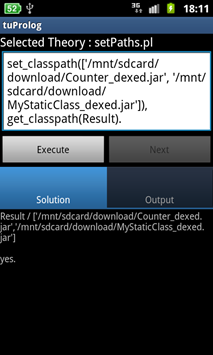
\includegraphics[height=200px]{images/android12.png}~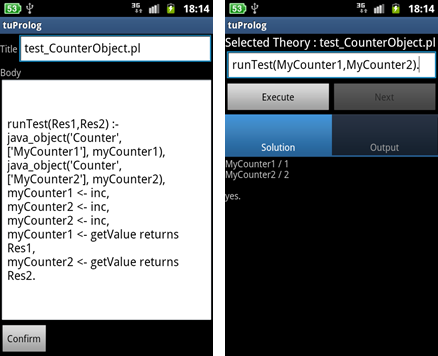
\includegraphics[height=200px]{images/android13.png}
  \caption{Managing class paths and objects via OOLibrary.}\label{fig:android12}
\end{figure}

%This behaviour has been tested on both virtual devices (Android 2.3.3 Gingerbread, Android 4.3 Jelly Bean) and some real devices (Samsung Galaxy W - Android 2.3.6 Gingerbread, Samsung Galaxy S3 Mini - Android 4.1.2 Jelly Bean, iOcean X7 - Android 4.2.1 Jelly Bean).

